%% Placeholder for chapter on convexity

%Below are notes for Oct23
\section{Linear/affine/convex/conic hulls \& sets}
Given a set of points $x^{(i)} \in \Re^n$, $i\in [m]$

\begin{equation*}
P = \{x^{(1)}, x^{(2)},..., x^{(m)} \}
\end{equation*}

Consider combinations of form $\sum^m_{i=1} \lambda_i x^{(1)}$

1) The "linear" hull: 

\begin{equation*}
\{x|x = \sum^m_{i=1} \lambda_i x^{(i)}, \lambda_r\in \Re, \forall i\in [m] \}
\end{equation*}

2) The "affine" hull: 

\begin{equation*}
\{x|x = \sum^m_{i=1} \lambda_i x^{(i)}, \lambda_i\in \Re, \sum^n_{i=1}\lambda_i = 1 \}
\end{equation*}


3) The "convex" hull: 

\begin{equation*}
\{x|x = \sum^m_{i=1} \lambda_i x^{(i)}, \lambda_i\in \Re, \lambda_i \geq 0, \sum^m_{i=1}\lambda_i = 1 \}
\end{equation*}


4) The "conic" hull: 

\begin{equation*}
\{x|x = \sum^m_{i=1} \lambda_i x^{(i)}, \lambda_i\in \Re, \lambda_i \geq 0 \}
\end{equation*}


\begin{center}
	\begin{tabular}{|c|c|c|}
	\hline  
   & $\lambda_i \geq 0$   & $\sum^m_{i=1}\lambda_i = 1$ \\
	\hline  
Linear&  no  & no \\
	\hline  
Affine&  no  &yes  \\
	\hline 
Covex&  yes  & yes \\
	\hline  
Conic&  yes  &  no\\
	\hline 
\end{tabular}
\end{center}



1) Linear Hull

Linear hull of $P = span\{x^{(1)},...,x^{(m)} \} =span(P)$

$\rightarrow$ smallest subspace that contains $P$.

2) Affine hull

\begin{align*}
P &= \{x^{(1)}, x^{(2)} \}\\
x &= \lambda_1x^{(1)} + \lambda_2x^{(2)}\\
&= \lambda_1x^{(1)} + (1-\lambda)_1x^{(1)}\\
&= x^{(2)} + \lambda(x^{(1)} - x^{(2)})\\
aff(P) &= x^{(2)} + span(x^{(1)} - x^{(2)})
\end{align*}

\begin{align*}
P &= \{x^{(1)}, x^{(2)}, x^{(3)} \}\\
x &= \lambda_1x^{(1)} + \lambda_2x^{(2)} + \lambda_3x^{(3)}\\
&= (1 - \lambda_2 - \lambda_3)x^{(1)} + \lambda_2x^{(2)} + \lambda_3x^{(3)}\\
&= x^{(1)} + \lambda_2(x^{(2)} - x^{(1)}) + \lambda_3(x^{(3)} - x^{(1)})
\end{align*}

\begin{marginfigure}
	\centering
	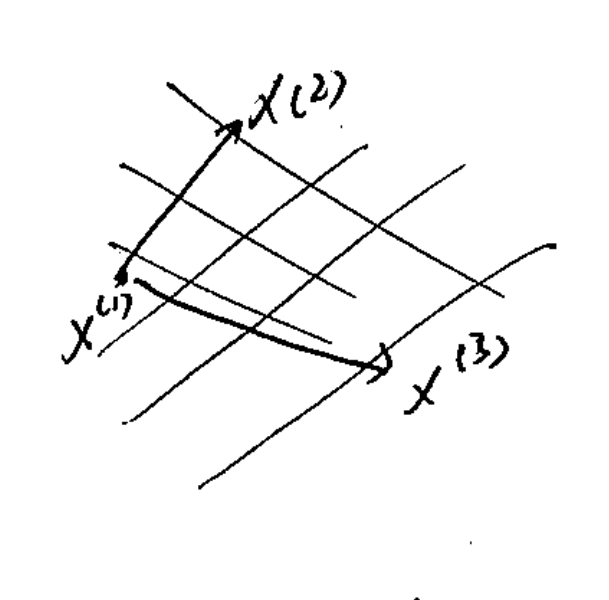
\includegraphics[width=1.8in,height=1.8in]{figures/ch08/figure1023_1.png}
	%\caption{This is an inserted JPG graphic} 
	%\label{fig:graph} 
\end{marginfigure}

3) Convex hulls

\begin{align*}
P &= \{x^{(1)},  x^{(2)}\}\\
x &= \lambda_1x^{(1)} + \lambda_2x^{(2)}\\
&= (1-\lambda)x^{(1)} + \lambda x^{(2)}\\
&= x^{(1)} + \lambda(x^{(2)} - x^{(1)})
\end{align*}

\begin{align*}
P &= \{x^{(1)},  x^{(2)}, x^{(3)} \}\\
x &= \lambda_1x^{(1)} + \lambda_2x^{(2)} + \lambda_3x^{(3)}\\
&= x^{(1)} + \lambda_2(x^{(2)} - x^{(1)}) + \lambda_3(x^{(3)} - x^{(1)})\\
&= x^{(1)} + \lambda \gamma(x^{(2)} - x^{(1)}) + (1 - \lambda)\gamma(x^{(3)} - x^{(1)})
\end{align*}


\begin{marginfigure}
	\centering
	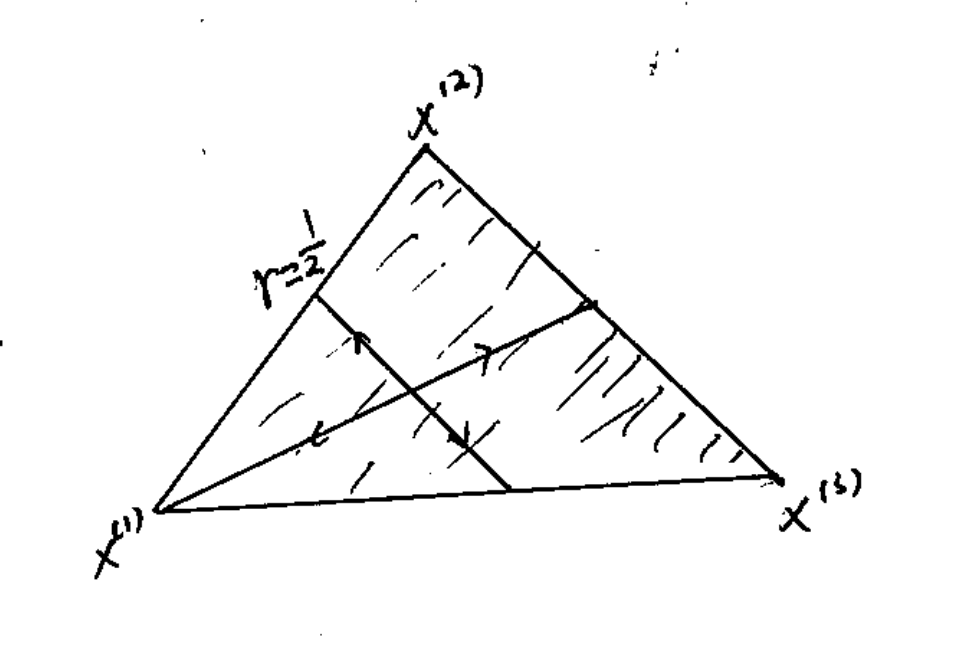
\includegraphics[width=1.8in,height=1.8in]{figures/ch08/figure1023_2.png}
	%\caption{This is an inserted JPG graphic} 
	%\label{fig:graph} 
\end{marginfigure}

\begin{marginfigure}
	\centering
	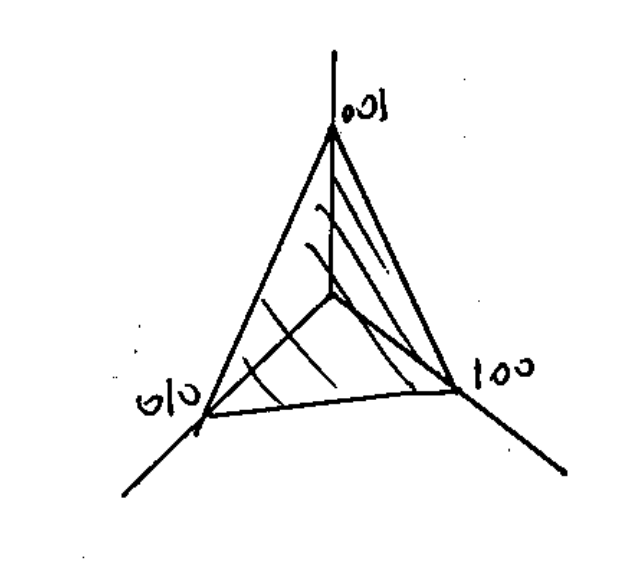
\includegraphics[width=1.8in,height=1.8in]{figures/ch08/figure1023_3.png}
	%\caption{This is an inserted JPG graphic} 
	%\label{fig:graph} 
\end{marginfigure}

4) Conic hulls: $\sum^n_{i=1}\lambda_i x^{(i)}$, $\lambda_i \geq 0$, $\forall i\in [m]$

\begin{align*}
P &= \{x^{(1)}, x^{(2)} \}\\
x &= \lambda_1x^{(1)} + \lambda_2x^{(2)}\\
&= ( \lambda_1 + \lambda_2)[\frac{\lambda_1}{\lambda_1 + \lambda_2}x^{(1)} + \frac{\lambda_2}{\lambda_1 + \lambda_2}x^{(2)}]\\
&= \gamma[\lambda x^{(1)} + (1-\lambda)x^{(2)}]
\end{align*}

\begin{marginfigure}
	\centering
	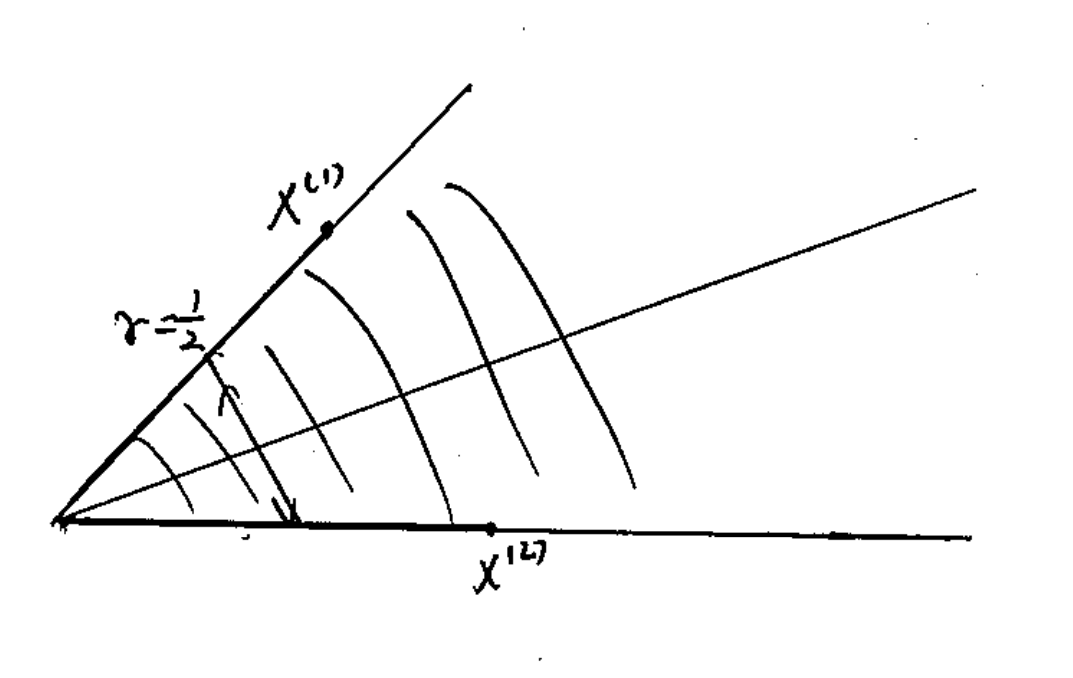
\includegraphics[width=1.8in,height=1.8in]{figures/ch08/figure1023_4.png}
	%\caption{This is an inserted JPG graphic} 
	%\label{fig:graph} 
\end{marginfigure}

\subsection{Convex Sets}

\begin{definition}{Convex}
	A subset $C\subseteq \Re^n$ is a "convex" set if $\forall x,y \in \mathcal{C}$, then $z\in \mathcal{C}$, $\forall z = \lambda x + (1-\lambda)y$, $\lambda \in [0,1]$
\end{definition}


\begin{definition}{Strictly Convex}
	A convex set is "strictly" convex if $\forall x,y \in \mathcal{C}$, $\forall \lambda \in (0,1)$, $z = \lambda x + (1-\lambda)y \in rel\,int(\mathcal{C})$(relative interior)
\end{definition}

Objects with straight edges are not strictly convex sets.

\begin{definition}{Cone}
	A set $\mathcal{C}\subseteq \Re^n $ is a cone if $\forall x\in \mathcal{C}$, then $\gamma x\in \mathcal{C}, \forall \gamma \geq 0$
\end{definition}

\begin{example}
	1) Hyper-planes are convex: $H = \{x| a^Tx = b \}$, pick $x,y \in H$, is $z =\lambda x + (1-\lambda)y \in H$? $\forall \lambda \in [0,1]$
	
	\begin{align*}
	a^Tz &= a^T(\lambda x + (1-\lambda)y)\\
	&= \lambda(a^Tx) + (1-\lambda)y\\
	&= \lambda b + (1-\lambda)b\\
	&= b
	\end{align*}
	
	
	2) Half-space: $\{x|a^Tx = b \}$, same proof except get inequality here in above equations($a^Tz \neq \lambda b + (1-\lambda)b$).
	
	3) If $c_1, ..., c_n$ al convex sets, then $\mathcal{C} = \cap^m_{i=1}$ is convex.
	
	\begin{proof}
		Pick any $x,y\in \mathcal{C}$ $\Rightarrow$ $x,y\in \mathcal{C}_i,\forall i\in [m]$.
		
		Consider any $z = \lambda x + (1 - \lambda)y$ , is this in $\mathcal{C}$?
		
		Since $x,y \in \mathcal{C}$, $\rightarrow z\in \mathcal{C}_i$ since $\mathcal{C}_i$, $\forall i\in [m]$
		
		If $z\in \mathcal{C}_i$, $\forall i\in [m]$ also intersection $\rightarrow z\in \cap^m_{i=1}C_i = C$
		
	\end{proof}

	In LP $\&$ QP Feasible set:
	
	\begin{equation*}
	\{x|Ax = b \}\cap \{x|Gx\leq b \} = \{\cap^q_{i=1}\{x|a^{(i)^T}x = b_i  \}\cap \{\cap^m_{i=1}\{x|g^{(i)^T}x \leq h_i \}
	\end{equation*}
	
	4) Affine transformations:
	
	If a map $F: \Re^n \rightarrow \Re^m$ is affine ($F(x) = Ax + b$) and $\mathcal{C} \subseteq \Re^n$ is convex, then the image of $\mathcal{C}$ under $F$ is convex.
	
	\begin{equation*}
	F(\mathcal{C}) = \{F(x) | x\in \mathcal{C} \} \subseteq \Re^m
	\end{equation*}

	Also pre-image of a convex set $\tilde{e}$ in $\Re^m$ is convex
	
	\begin{equation*}
	\{x|F(x)\in \mathcal{C} \} \subseteq \Re^n
	\end{equation*}
\end{example}

\begin{marginfigure}
	\centering
	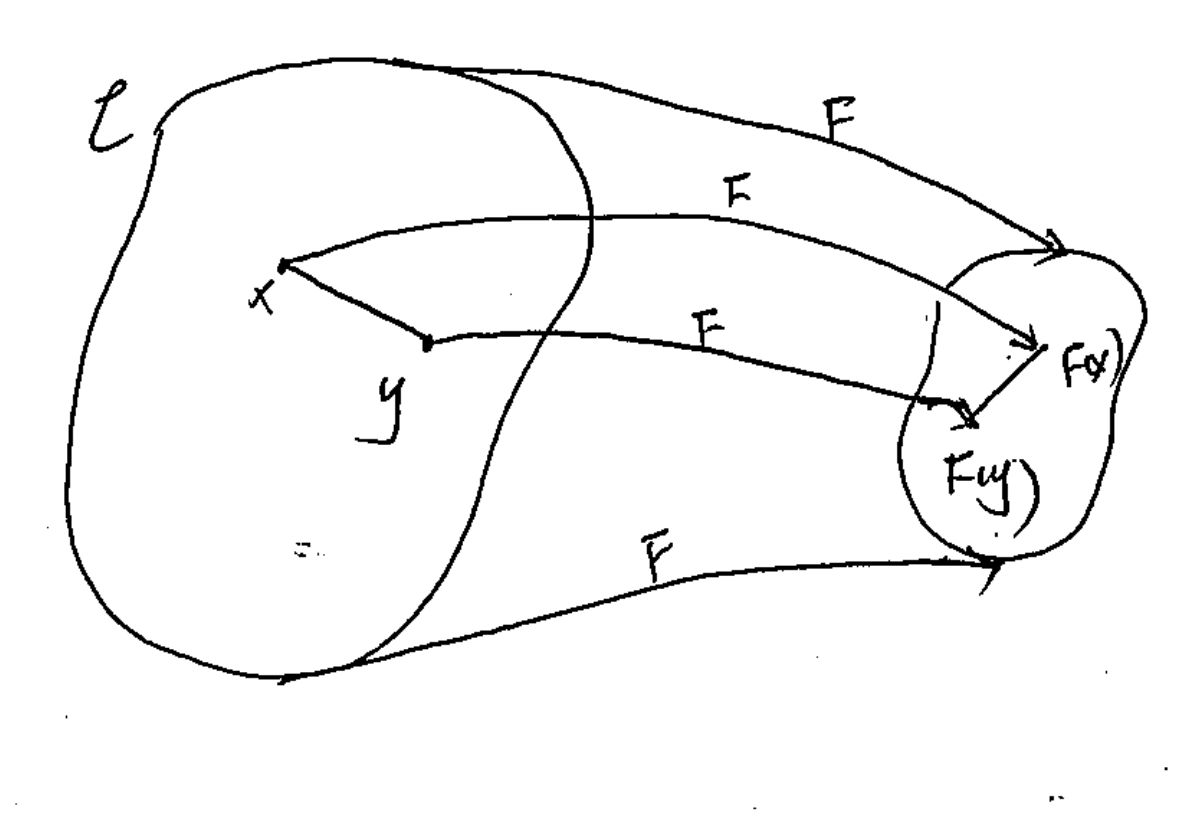
\includegraphics[width=1.8in,height=1.8in]{figures/ch08/figure1023_5.png}
	%\caption{This is an inserted JPG graphic} 
	%\label{fig:graph} 
\end{marginfigure}


Norm balls are convex

\begin{marginfigure}
	\centering
	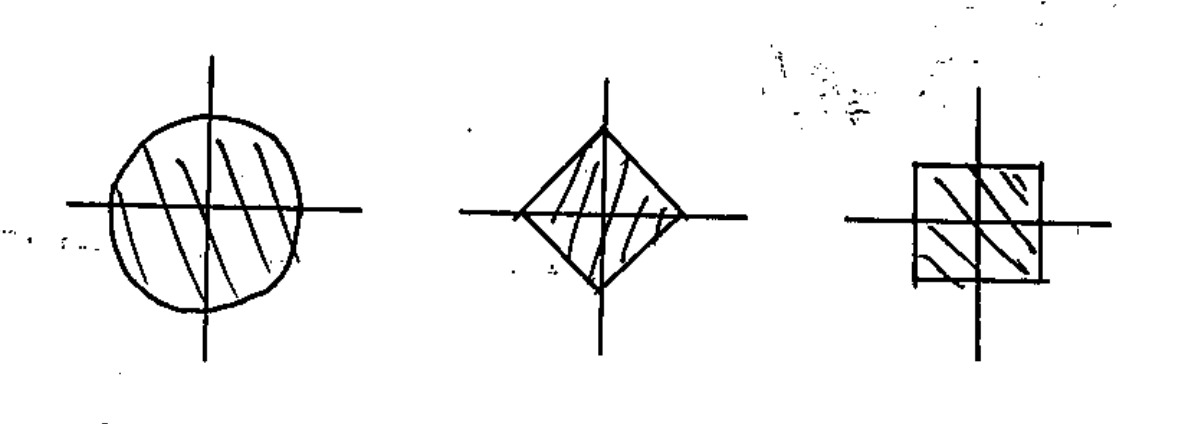
\includegraphics[width=1.8in,height=1.8in]{figures/ch08/figure1023_6.png}
	%\caption{This is an inserted JPG graphic} 
	%\label{fig:graph} 
\end{marginfigure}

\begin{proof}
	Take any two points $u,v$ s.t. $\Vert u\Vert \leq 1$, $\Vert v\Vert \leq 1$. 
	
	\begin{align*}
	\Vert \lambda u+(1-\lambda)v\Vert &\leq \Vert \lambda u\Vert + \Vert (1-\lambda)v\Vert\\
	&= \vert \lambda \vert \Vert  u\Vert + \vert (1-\lambda) \vert \Vert  v\Vert\\
	&= \lambda\Vert  u\Vert + (1-\lambda)\Vert  v\Vert\\
	&\leq \lambda 1 + (1-\lambda)1\\
	&= 1
	\end{align*}
	
	\begin{equation*}
	\Vert  x\Vert_p = (\sum^n_{i=1}\vert  x_i\vert^p)^{\frac{1}{p}}
	\end{equation*}
	norm if $p\geq 1$
\end{proof}

\subsection{Ellipsoids}

\begin{equation*}
\xi(x_c, P) =\{x|(x - x_c)^TP^{-1}(x - x_c) \leq 1 \}
\end{equation*}
where $P\in S^n_{++}$   is a convex set.

\begin{proof}
	
	$l_2$ norm ball is convex. 
	
	Consider following affine map $F(u) = P^{\frac{1}{2}}u + x_c$.
	
	The set $\{F(u) | \Vert y\Vert_2 \leq 1 \}$ is convex. 
\end{proof}

Define a set:

\begin{align*}
\{F(u) | \Vert u\Vert^2_2 \leq 1 \} &= \{x|x = P^{\frac{1}{2}}u+x_c, \Vert u\Vert^2 \leq 1 \}\\
&= \{x|x - x_c = P^{\frac{1}{2}}u, \Vert u\Vert^2 \leq 1 \}\\
&= \{x|P^{-\frac{1}{2}}(x - x_c) =u, \Vert u\Vert^2 \leq 1 \}\\
&= \{x|\Vert P^{-\frac{1}{2}}(x - x_c)\Vert^2_2 \leq 1 \}\\
&= \{x|(x - x_c)^TP^{-1}(x - x_c) \leq 1 \}
\end{align*}

Intersect these shapes with polyhedron to get feasible set of QCQP.

\begin{example}
	\begin{align*}
	\{x | \Vert Ax - b \Vert^2_2 \leq 1 \} &= \{x | \Vert F(x) \Vert^2 \leq 1 \}  where F(x) = Ax - b
	\end{align*}
	
	Pre-image of convex set under an affine function and so it's convex
\end{example}


%Above are notes for Oct23


%Below are notes for Oct30
Consider an affine function $F(x) = Ax + b$, $A\in \Re^{m\times n}$, $b\in \Re^m$, $F:\Re^n \rightarrow \Re^m$

Then:

\begin{enumerate}
	\item $\forall \mathcal{C}\subseteq \Re^n$ that are convex, the image of $\mathcal{C}$ under action of $F$ is a convex set in $\Re^m$:
	
	\begin{equation*}
	F(\mathcal{C}) = \{F(x)\in \Re^m \vert x\in \mathcal{C} \}
	\end{equation*}
	
	\item $\forall \mathcal{C}\subseteq \Re^m$ that are convex, the pre-image ("inverse image") of $\mathcal{C}$ under $F$: 
	\begin{equation*}
	F^{-1}(\mathcal{C}) = \{x| F(x)\in \mathcal{C} \}
	\end{equation*}
	is a convex set $\in \Re^n$
\end{enumerate}

Used (1) show:
\begin{itemize}
	\item all norm balls are convex sets.
	
	\item ellipsoids are convex sets.
\end{itemize}

\begin{example}
	$\{x|\Vert Ax + b\Vert \leq 1 \}$ is a convex set$\rightarrow$ 
	
	Let $F(x) = Ax + b$(affine function)
	
	Let $\beta = \{x|\Vert x \Vert \leq 1 \}\in \Re^m$
	
	\begin{align*}
	\{x|\Vert Ax+b\Vert\leq 1 \} &= \{x|\Vert F(x) \Vert\leq 1 \}\\
	&= \{x|F(x) \leq \beta \}\\
	&= F^{-1}(\beta)
	\end{align*}
\end{example}


Recall:

$\mathcal{C}$ is a cone if $\forall x\in \mathcal{C}$ and $\theta \in \Re_{+}$(i,e. $\theta \geq 0$)   

Important cones: PSD matrices   


\begin{align*}
S^n &= \{x\in \Re^{n\times n}s.t. x = x^T \}\\
S^n_+ &= \{x\in S^{n}s.t. v^TXv \geq 0, \forall v\in \Re^n \}\\
S^n &= \{x\in S^{n}s.t. v^TXv > 0 ,\forall v\in \Re^n\}
\end{align*}

1) $S_+^n$ is a cone since $\forall x \in S_+^n$ and $\forall \theta \geq 0$:

\begin{equation*}
v^T(\theta X)v = \theta v^TXv  > 0
\end{equation*}

write:
\begin{align*}
X\in S^n_+ &\Leftrightarrow X\geq 0\\
X\in S^n_{++} &\Leftrightarrow X> 0
\end{align*}

2) $S_+^n$ is a convex cone.

Let $A\in S^n_+$, $B\in S^n_+$ consider $\lambda A + (1-\lambda)B$ where $\lambda \in [0,1]$

$\rightarrow$ First note $(\lambda A + (1-\lambda)B)^T= \lambda A^T + (1-\lambda)B^T = \lambda A + (1-\lambda)B \in S^n$


$\rightarrow$ $v^T(\lambda A + (1-\lambda B)v) =\lambda(v^TAv) + (1-\lambda)(v^TBv)\geq 0$\\
 
3) Statements for $S^n_{++}$ follow with $>$ rather than $\geq$

Cones lead to "generalized" inequalities.

Want to extend idea of orderings to $\Re^n$

Start with a "proper" cone $K\in \Re^n$:
\begin{itemize}
	\item closed, convex
	
	\item non-empty("solid")
	
	\item "pointed"(doesn't contain lines)
\end{itemize}


A proper cone $K$ defines a generalized inequality $\leq_K$: "less-than-or-equal to with respect to cone $K$"

How to interpret $\leq_K$:

\begin{align*}
x\leq_K y &\Leftrightarrow 0\leq_K (y-x)\Leftrightarrow y - x \in K\\
x <_K &\Leftrightarrow y-x\in int(K)
\end{align*}

\begin{marginfigure}
	\centering
	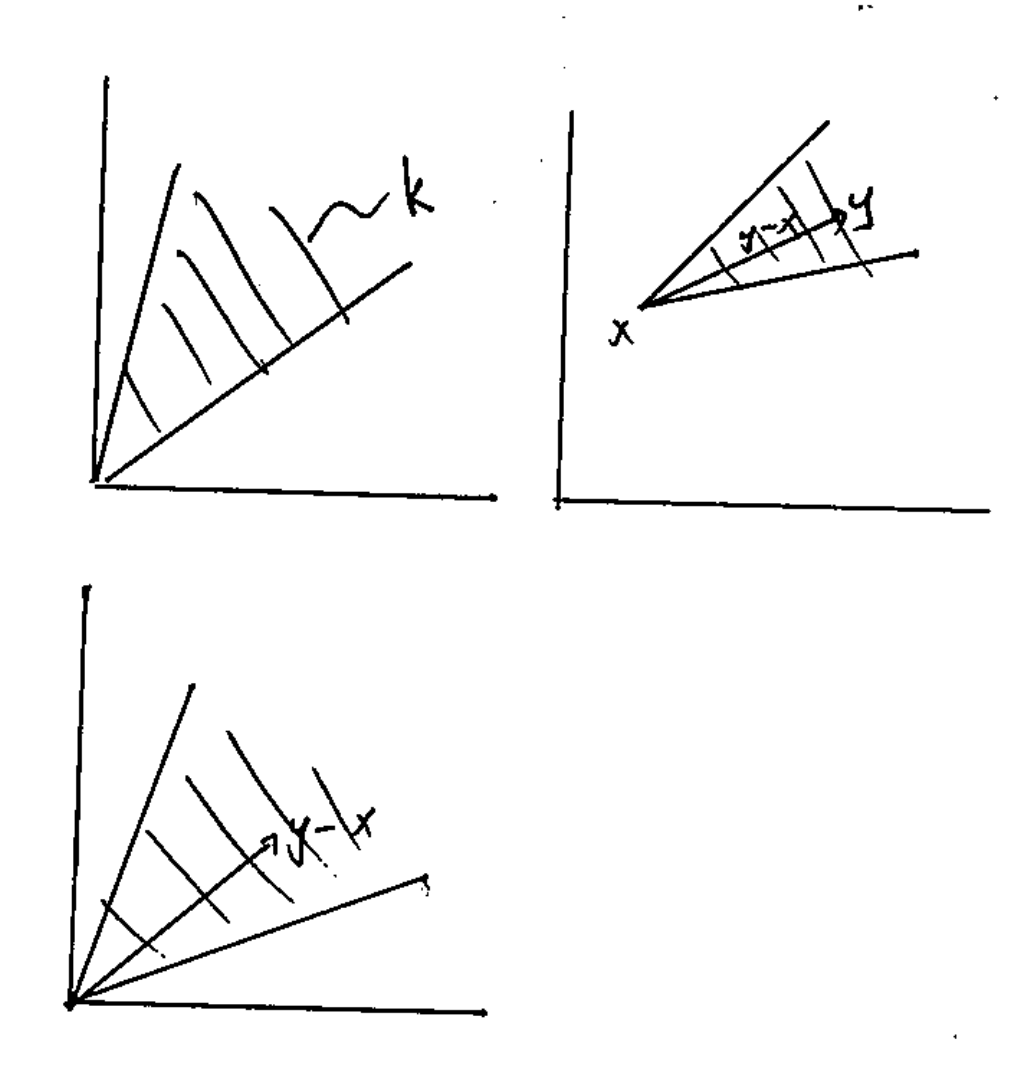
\includegraphics[width=1.8in,height=1.8in]{figures/ch08/figure1030_1.png}
	%\caption{This is an inserted JPG graphic} 
	%\label{fig:graph} 
\end{marginfigure}


\begin{example}
	$k = S^n_+$ ordering of matrices, elements of vector space are in $S^n$
	
	$X\leq_k y$ means $y-x\in S^n_+	$
	
	$\rightarrow$ is it true that $v^T(y-x)x \geq 0$, $\forall v$
	
	$\rightarrow$ are all eigenvalues non-negative
	
	Note: Interior of $S_+^n$ is $S^n_{++}$
	
	$x\leq_{S^n_+}y$
\end{example}

The 2 generalized inequalities come up so often, they are default.

\begin{enumerate}
	\item If compare 2 vectors $x,y\in \Re^n$, write $x\leq  y\Leftrightarrow x\leq_{\Re^n_{+}}y \Leftrightarrow y-x\in \Re^n_{+}$ 
	
	\item If compare 2 symmetric matrices, write:
	
	\begin{align*}
	x\leq y &\Leftrightarrow x\leq_{S_+^n} y\Leftrightarrow y - x\in S^n_{++}\\
	x< y &\Leftrightarrow y - x\in S^n_{+}
	\end{align*}
\end{enumerate}

\begin{example}
	$\{x\in \Re^n | x_1A_1 + x_2A_2 + ... + x_nA_n \leq B\}$
\end{example}

where $A_i\in S^m$ $B\in S^m$

"linear matrix inequality"

$F(x) = B - \sum^n_{i=1}x_iA_i$ $\leftarrow$affine function of $x$

\begin{align*}
\{x\in \Re^n | x_1A_1 + x_2A_2 + ... + x_nA_n \leq B\}
 &= \{x\in \Re^n | F(x)\geq 0\}\\
 &= \{x\in \Re^n | F(x)\in S^n_+ \}\\
 &=F^{-1}(S^n_+)
\end{align*}
So, a convex set.\\


Properties of Convex Sets:


\begin{marginfigure}
	\centering
	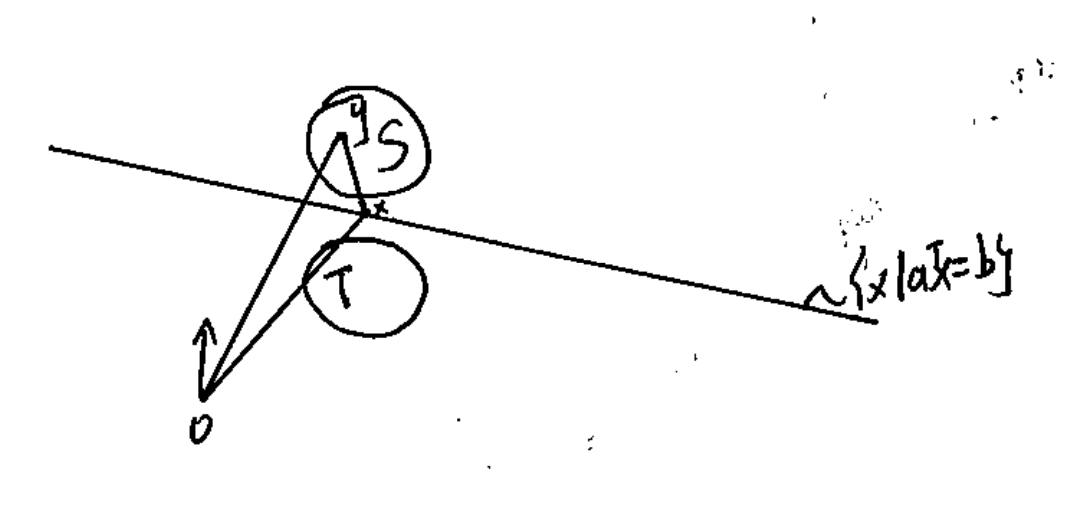
\includegraphics[width=1.8in,height=1.8in]{figures/ch08/figure1030_2.png}
	%\caption{This is an inserted JPG graphic} 
	%\label{fig:graph} 
\end{marginfigure}


\begin{enumerate}
	\item Separating hyperplane: If $S,T$ are convex sets in $\Re^n$ and disjoint, i.e, $S\cap T = \emptyset$, then there exists an $a \in \Re^n$ and $a,b\in \Re$ s.t.
	
	\begin{align*}
	a^Tx&\geq b, \forall x\in S\\
	a^Tx &<b, \forall x\in T
	a^Ty - a^Tx &= a^T(y-x) \geq 0
	\end{align*}
	
	\item Supporting hyperplanes:
	
	If $S$ is a convex set then $\forall x_0\in \delta \mathcal{S}$(boundary of $S$), $\exists a\in \Re^n$ s.t. 
	\begin{align*}
	a^Tx \leq a^Tx_0\\
	a^T(x - x_0)\leq 0
	\end{align*}
	
	\begin{marginfigure}
	\centering
	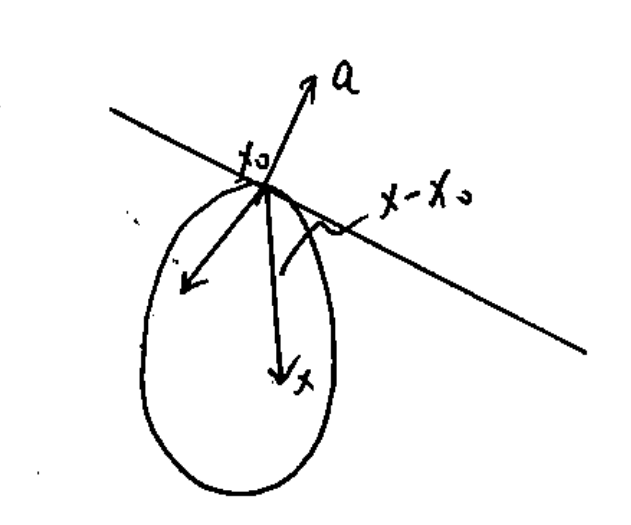
\includegraphics[width=1.8in,height=1.8in]{figures/ch08/figure1030_3.png}
	%\caption{This is an inserted JPG graphic} 
	%\label{fig:graph} 
	\end{marginfigure}
	
	\begin{marginfigure}
	\centering
	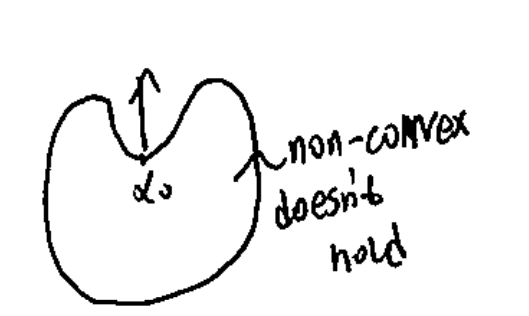
\includegraphics[width=1.8in,height=1.8in]{figures/ch08/figure1030_4.png}
	%\caption{This is an inserted JPG graphic} 
	%\label{fig:graph} 
	\end{marginfigure}
	
	\begin{marginfigure}
	\centering
	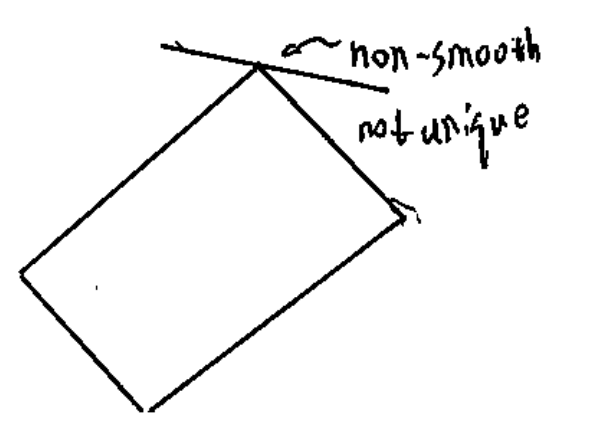
\includegraphics[width=1.8in,height=1.8in]{figures/ch08/figure1030_5.png}
	%\caption{This is an inserted JPG graphic} 
	%\label{fig:graph} 
	\end{marginfigure}
\end{enumerate}

\subsection{Convex Functions}
Let $F$ have aconvex domain, then $F:\Re^n\rightarrow \Re$ a convex function if $\forall x,y \in dom(F)$:

\begin{equation*}
F(\lambda x + (1-\lambda)y) \leq \lambda F(x) + (1-\lambda)F(y), \forall \lambda \in [0,1]
\end{equation*}

and strictly convex if 
\begin{equation*}
F(\lambda x + (1-\lambda)y) < \lambda F(x) + (1-\lambda)F(y), \forall \lambda \in (0,1)
\end{equation*}
.
Note: $F$ is a "concave" if $-F$ is convex.

\begin{marginfigure}
	\centering
	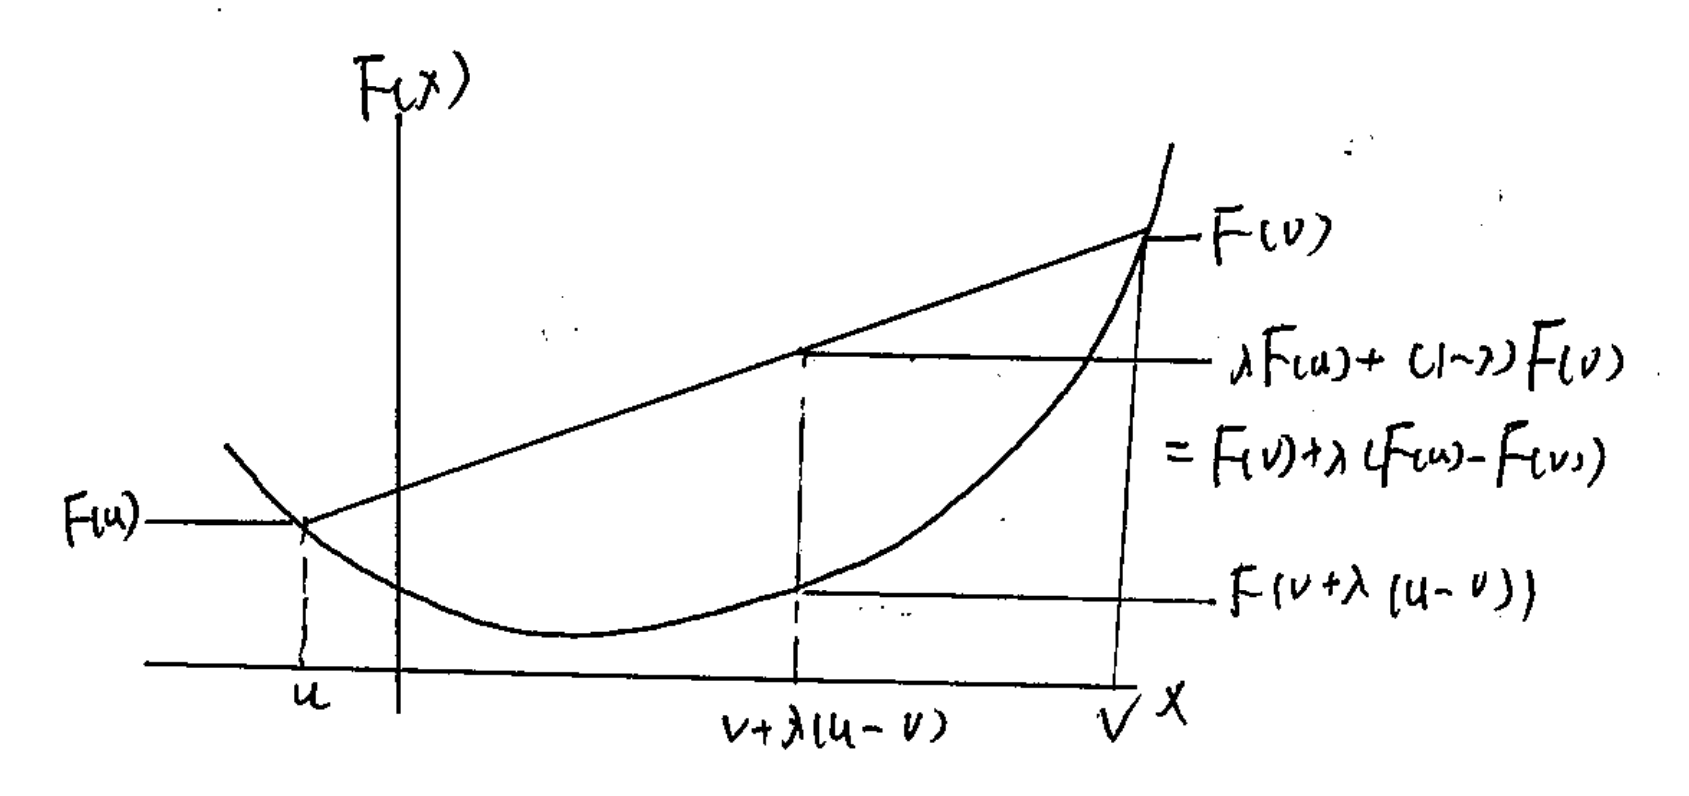
\includegraphics[width=1.8in,height=1.8in]{figures/ch08/figure1030_6.png}
	%\caption{This is an inserted JPG graphic} 
	%\label{fig:graph} 
\end{marginfigure}

Definition of convex:

\begin{equation*}
F(\lambda u + (1-\lambda)v) \leq \lambda F(u) + (1-\lambda)F(v)
\end{equation*}

And $F(\lambda u + (1-\lambda)v)$ can be written as $F(v + \lambda(u-v))$:

\begin{equation*}
F(\lambda u + (1-\lambda)v) \leq \lambda F(v) + \lambda(F(u)-F(v))
\end{equation*}

line segment connecting $(u,F(u))$ to $(v, F(v))$ always above buttom of bawl.


Sometimes define an "extended value" function

$$ \tilde{F}(x)=\left\{
\begin{array}{rcl}
F(x)       &      & \text{if } x\in dom(F)\\
\infty   &      & else
\end{array} \right. 
$$

Give an example:
\begin{itemize}
	\item Linear and affine
	
	\begin{marginfigure}
	\centering
	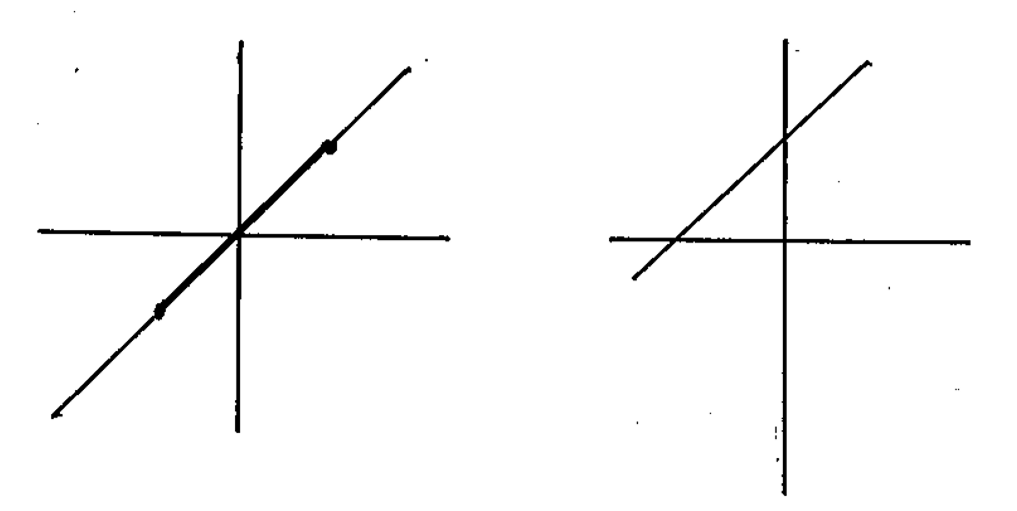
\includegraphics[width=1.8in,height=1.8in]{figures/ch08/figure1030_7.png}
	%\caption{This is an inserted JPG graphic} 
	%\label{fig:graph} 
	\end{marginfigure}
	
	both convex \& concave
	
	\item $x^2$ convex
	
	\begin{marginfigure}
	\centering
	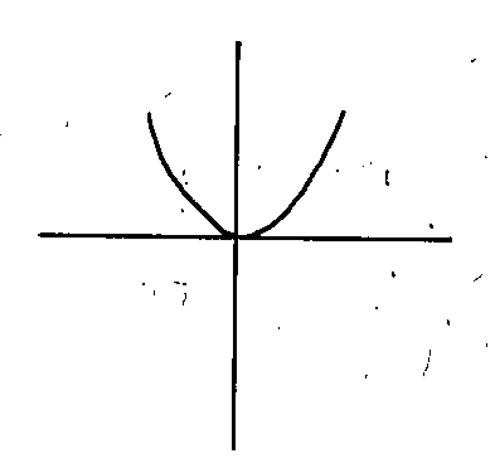
\includegraphics[width=1.8in,height=1.8in]{figures/ch08/figure1030_8.png}
	%\caption{This is an inserted JPG graphic} 
	%\label{fig:graph} 
	\end{marginfigure}
	
	\item $F(x) = logx$ with $domF = \Re_{++}$, concave
	
	\begin{marginfigure}
	\centering
	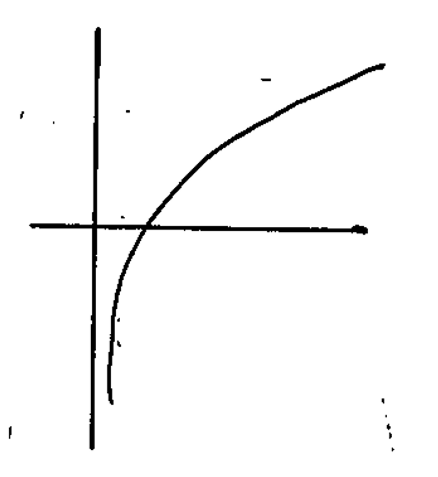
\includegraphics[width=1.8in,height=1.8in]{figures/ch08/figure1030_9.png}
	%\caption{This is an inserted JPG graphic} 
	%\label{fig:graph} 
	\end{marginfigure}
	
	\item $\Vert x\Vert$ is convex:
	
	\begin{align*}
	\Vert \lambda x + (1-\lambda)y\Vert &\leq \Vert \lambda x\Vert + \Vert(1-\lambda)y\Vert\\
	&= \lambda \Vert x \Vert + (1-\lambda)\Vert y \Vert
	\end{align*}
	
	\item $\frac{1}{x}$ convex on $\Re_{++}$, concave on $\Re_{--}$
	
	\begin{marginfigure}
	\centering
	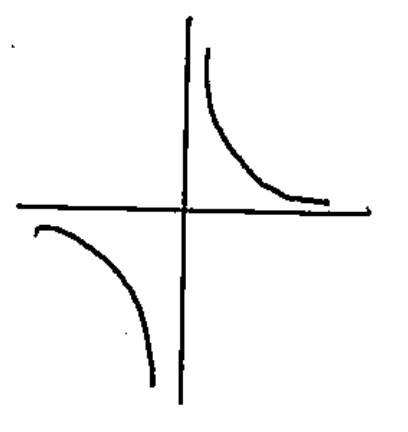
\includegraphics[width=1.8in,height=1.8in]{figures/ch08/figure1030_10.png}
	%\caption{This is an inserted JPG graphic} 
	%\label{fig:graph} 
	\end{marginfigure}
\end{itemize}

Recall: Epigraph of a function

\begin{equation*}
epiF = \{(x,t)|t\geq F(x), x\in domF \}
\end{equation*}

\begin{marginfigure}
	\centering
	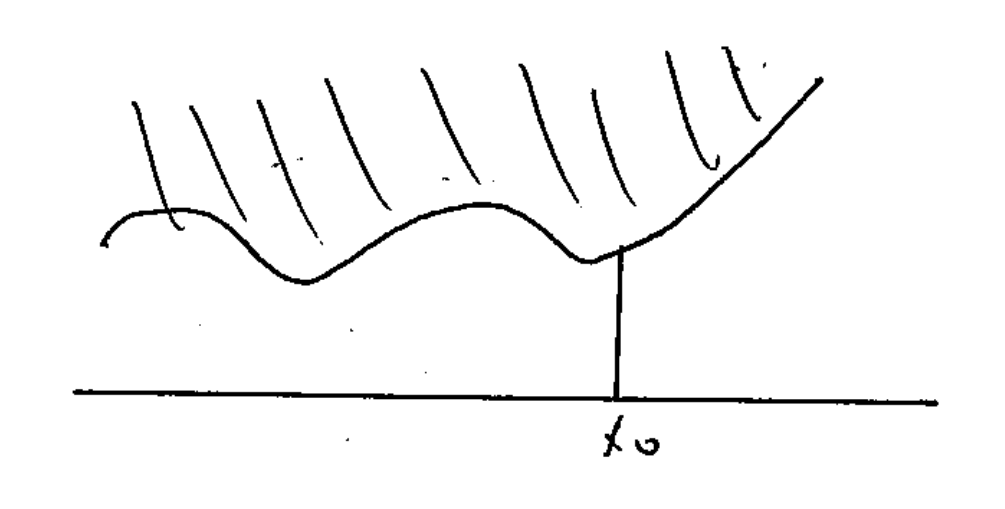
\includegraphics[width=1.8in,height=1.8in]{figures/ch08/figure1030_11.png}
	%\caption{This is an inserted JPG graphic} 
	%\label{fig:graph} 
\end{marginfigure}

\begin{definition}
	$f$ is a convex function iff $epif$ is a convex set
\end{definition}

\begin{definition}{Sublevel sets}
	$\mathcal{C}(\alpha) = \{x|F(x)\leq \alpha, x\in domF \}$.
	
	\begin{marginfigure}
	\centering
	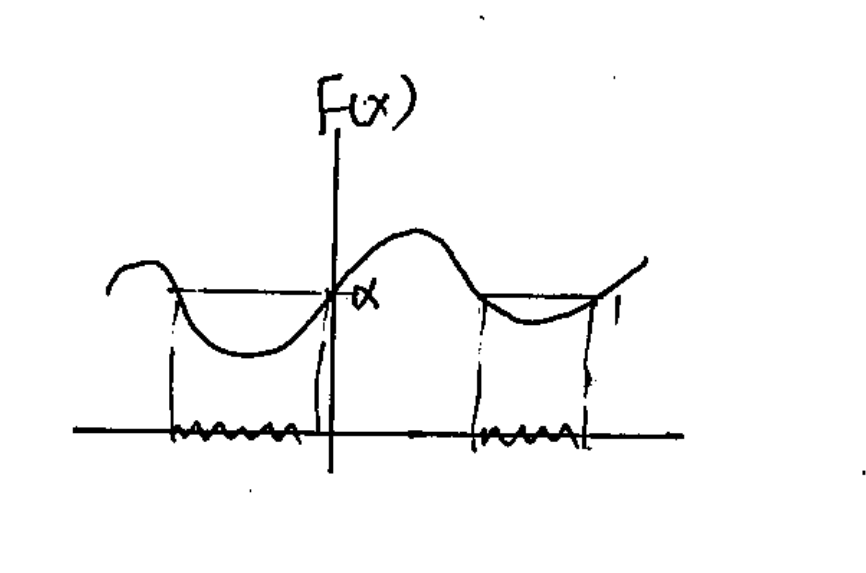
\includegraphics[width=1.8in,height=1.8in]{figures/ch08/figure1030_12.png}
	%\caption{This is an inserted JPG graphic} 
	%\label{fig:graph} 
	\end{marginfigure}
\end{definition}

\begin{theorem}
	If $F$ is convex, its sub-level sets are all convex sets.
\end{theorem}

Converse is nor true $\rightarrow$ if all sub-level sets of a function are convex sets, the function is "quasi-convex" but not necessarily convex.\\

\begin{marginfigure}
	\centering
	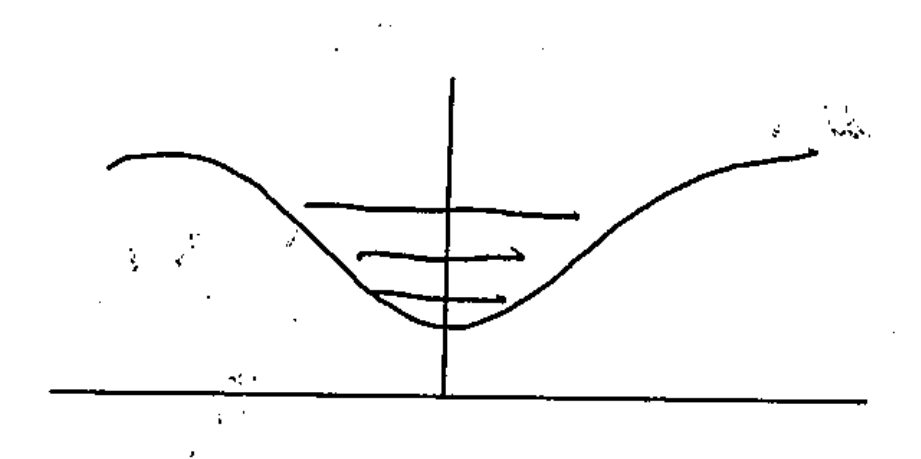
\includegraphics[width=1.8in,height=1.8in]{figures/ch08/figure1030_13.png}
	%\caption{This is an inserted JPG graphic} 
	%\label{fig:graph} 
\end{marginfigure}

1) Non-negative sums of convex functions are convex.

Let $F(x) =\sum^m_{i=1}a_iF_i(x)$, $domF = \cap^m_{i=1}domF_i$. 

\begin{align*}
F(\lambda x + (1-\lambda)y) &= \sum^m_{i=1}a_iF_i(\lambda x + (1-\lambda)y)\\
&\leq \sum^m_{i=1}a_i[\lambda F_i(x) + (1-\lambda)F_i(y)]\\
&= \lambda[\sum^m_{i=1}a_iF_i(\lambda)] + (1-\lambda)[\sum^m_{i=1}a_iF_i(y)]
\end{align*}

2) Convex functions of affine transformations of variables

Let $g(x) =F(Ax + b)$ where $F(\cdot)$ is convex.

\begin{align*}
g(\lambda x + (1-\lambda)y) &= F(A(\lambda x + (1-\lambda)y) + b)\\
&= F(\lambda(Ax + b) + (1-\lambda)F(Ay+b))\\
&\leq \lambda F(Ax + b) + (1-\lambda)F(Ay+b)\\
&= \lambda g(\lambda) + (1-\lambda)g(y)
\end{align*}

\begin{equation*}
dom(g) = \{x|Ax + b \in domF \}
\end{equation*}


3) The max of a pair of convex functions is a convex function:

\begin{equation*}
g(x) = max\{F_1(x), F_2(x) \}
\end{equation*}


\begin{marginfigure}
	\centering
	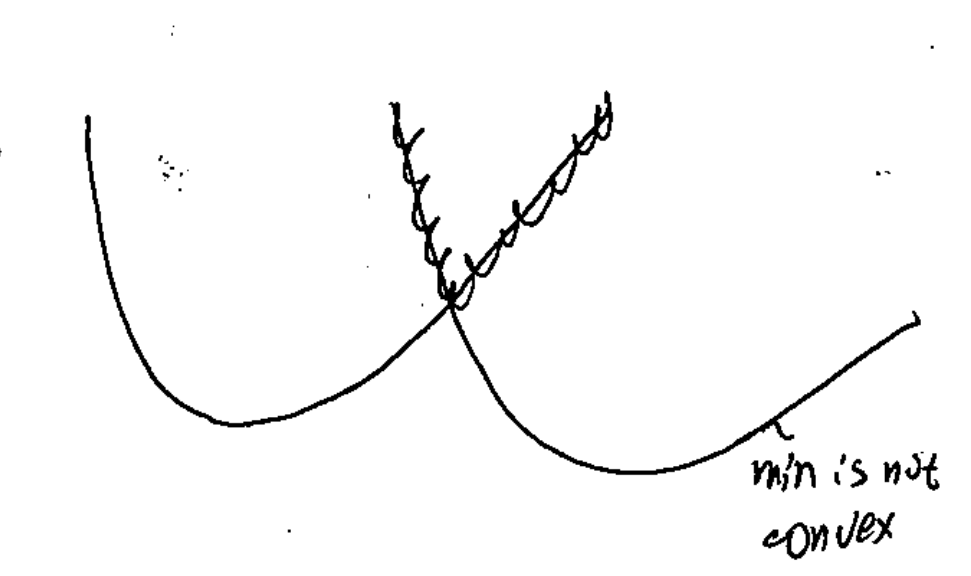
\includegraphics[width=1.8in,height=1.8in]{figures/ch08/figure1030_14.png}
	%\caption{This is an inserted JPG graphic} 
	%\label{fig:graph} 
\end{marginfigure}
%Above are notes for Oct30

%Below are notes for Nov 4

%Above are notes for Nov 4
